\chapter{Baza de date}

În acest capitol este argumentată alegerea unui tip de baze de date SQL, mai exact MySQL, pentru a reține informații importante aplicației. A fost preferată o abordare clasică asupra unei baze de date relaționale în special datorită numărului mare de tranzacții ce necesită o asigurare mai mare a integrității datelor \cite{sql1}.

Aplicația \thesistitle este de tip utilitar, aceasta are scopul de a fi folosită într-un context restrâns, în cadrul facultății. Prin urmare numărul de utilizatori este unul relativ mic, reprezentat de către studenți și profesori. De asemenea, poate fi observată o relație strânsă între profesori și propunerile acestora, dar și între studenți și preferințele acestora.

Relațiile între entități sunt de mai multe tipuri, în special \textit{One-to-one} și \textit{One-to-many}. Acest lucru se poate observa în diagrama următoare a bazei de date utilizate.

\begin{figure}[H]
	\centering
	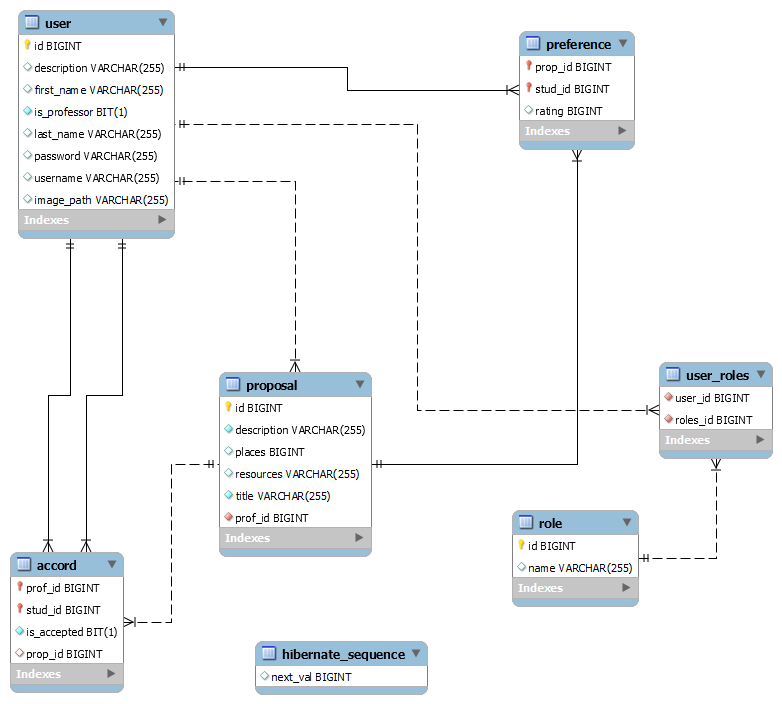
\includegraphics[width=\textwidth, left]{DB_diagram.png}
	\caption{Baza de date}
\end{figure}

În următoarele subcapitole sunt detaliate modelele utilizate pentru a reprezenta aceste date.

\section{Modelarea utilizatorilor}

Utilizatorii au fost modelați într-un mod clasic. Aceștia au la rândul lor roluri în funcție de drepturile pe care le au ei în cadrul aplicației. Astfel, sunt identificate două astfel de roluri: \textbf{ROLE\_USER} și \textbf{ROLE\_ADMIN}. Pe lângă acest lucru, utilizatorii sunt ori profesori, ori studenți, particularitate ilustrată de câmpul boolean \textit{is\_professor} al entității \texttt{user}.

\begin{figure}[H]
	\centering
	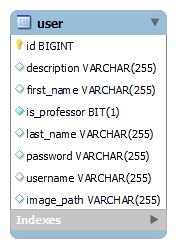
\includegraphics[width=0.4\textwidth, center]{user_model.png}
	\caption{Baza de date}
\end{figure}

Fiecare utilizator este identificat unic printr-un \texttt{id} de tipul de date BIGINT, care este și cheie primară a entității. Ca în majoritatea cazurilor, aceștia au un nume de familie (\texttt{last\_name}) și un prenume (\texttt{first\_name}). Câmpul \texttt{username} este de tipul VARCHAR(255) și este reprezentat de un email valid, lucru asigurată pe partea de front-end. Câmpul \texttt{password} este tot de tipul VARCHAR(255) și reprezintă parola utilizatorului, însă criptată pe partea de back-end cu un algoritm clasic.
Aceste două câmpuri sunt primite de către utilizator din partea unui administrator și sunt utilizate pentru autentificarea în aplicație. A fost preferată această abordare pentru a împiedica crearea de conturi din partea unor persoane din afara contextului.

\subsection{ROLE\_USER}

Cei mai mulți utilizatori au rolul \textbf{ROLE\_USER}, un rol default. Acest lucru le autorizează accesul la aplicație, odată ce aceștia sunt autentificați. Interfața diferă în funcție de tipul utilizatorului.

\subsubsection{Tipuri}

\textbf{Profesorii} pot crea și actualiza propuneri (en. proposals) pentru teza de licență. Aceste propuneri pot fi \textit{project} sau \textit{topic}, detalierea acestora urmând a fi făcută ulterior. De asemenea, aceștia pot încheia acorduri (en. accords) cu anumiți studenți pentru unele dintre propunerile lor. Acest lucru le permite studenților să nu mai participe la algoritmul de stable matching, fiind deja repartizați profesorilor respectivi.

La nivelul bazei de date, fiecare profesor are și un grad academic, reprezentat în tabela auxiliara \texttt{professor} prin \texttt{rank}.

\textbf{Studenții} pot crea și actualiza preferințe (en. preferences) într-o anumită ierarhie a lor. Așadar, categorisirea utilizatorilor în profesori și studenți are unicul scop de a diferenția interfața în funcție de funcționalitățile specifice tipurilor acestora.

Pe lângă câmpurile specifice unui utilizator, fiecare student are și un număr matricol reținut în câmpul \texttt{reg\_no} din tabela \texttt{student}.

\subsection{ROLE\_ADMIN}

Există în plus un număr restrâns de utilizatori care au rolul de administrator, \textbf{ROLE\_ADMIN}. Aceștia au dreptul de a gestiona conturile participanților, mai precis de a crea, actualiza și elimina utilizatorilor. De asemenea, administratorii au opțiunea de a impune anumite limite în cadrul aplicației cum ar fi o limită a propunerilor pentru profesori și o limită a preferințelor pentru elevi.

\section{Preferințele}

\section{Propunerile}

\section{Acordurile}